\chapter{Game Design}
\todo{don't just document the design, but also the decisions behind it}

- We want the game to be good, so we should think about the things that will make it good. It is for a specific audience.

\section{Design goals}

- these are the goals the game should achieve (each will have explanation --- what and why)

1. strategic depth in each battle

2. strategic depth in each run

3. make various strategies viable

4. force exploration

5. provide a challenge

- some of our goals are achieved very well in other games of the relevant genres, so we can look at them for inspiration

\subsection{Slay the Spire}

- explain the game, use the following images

\begin{figure}[htb]
    \centering
    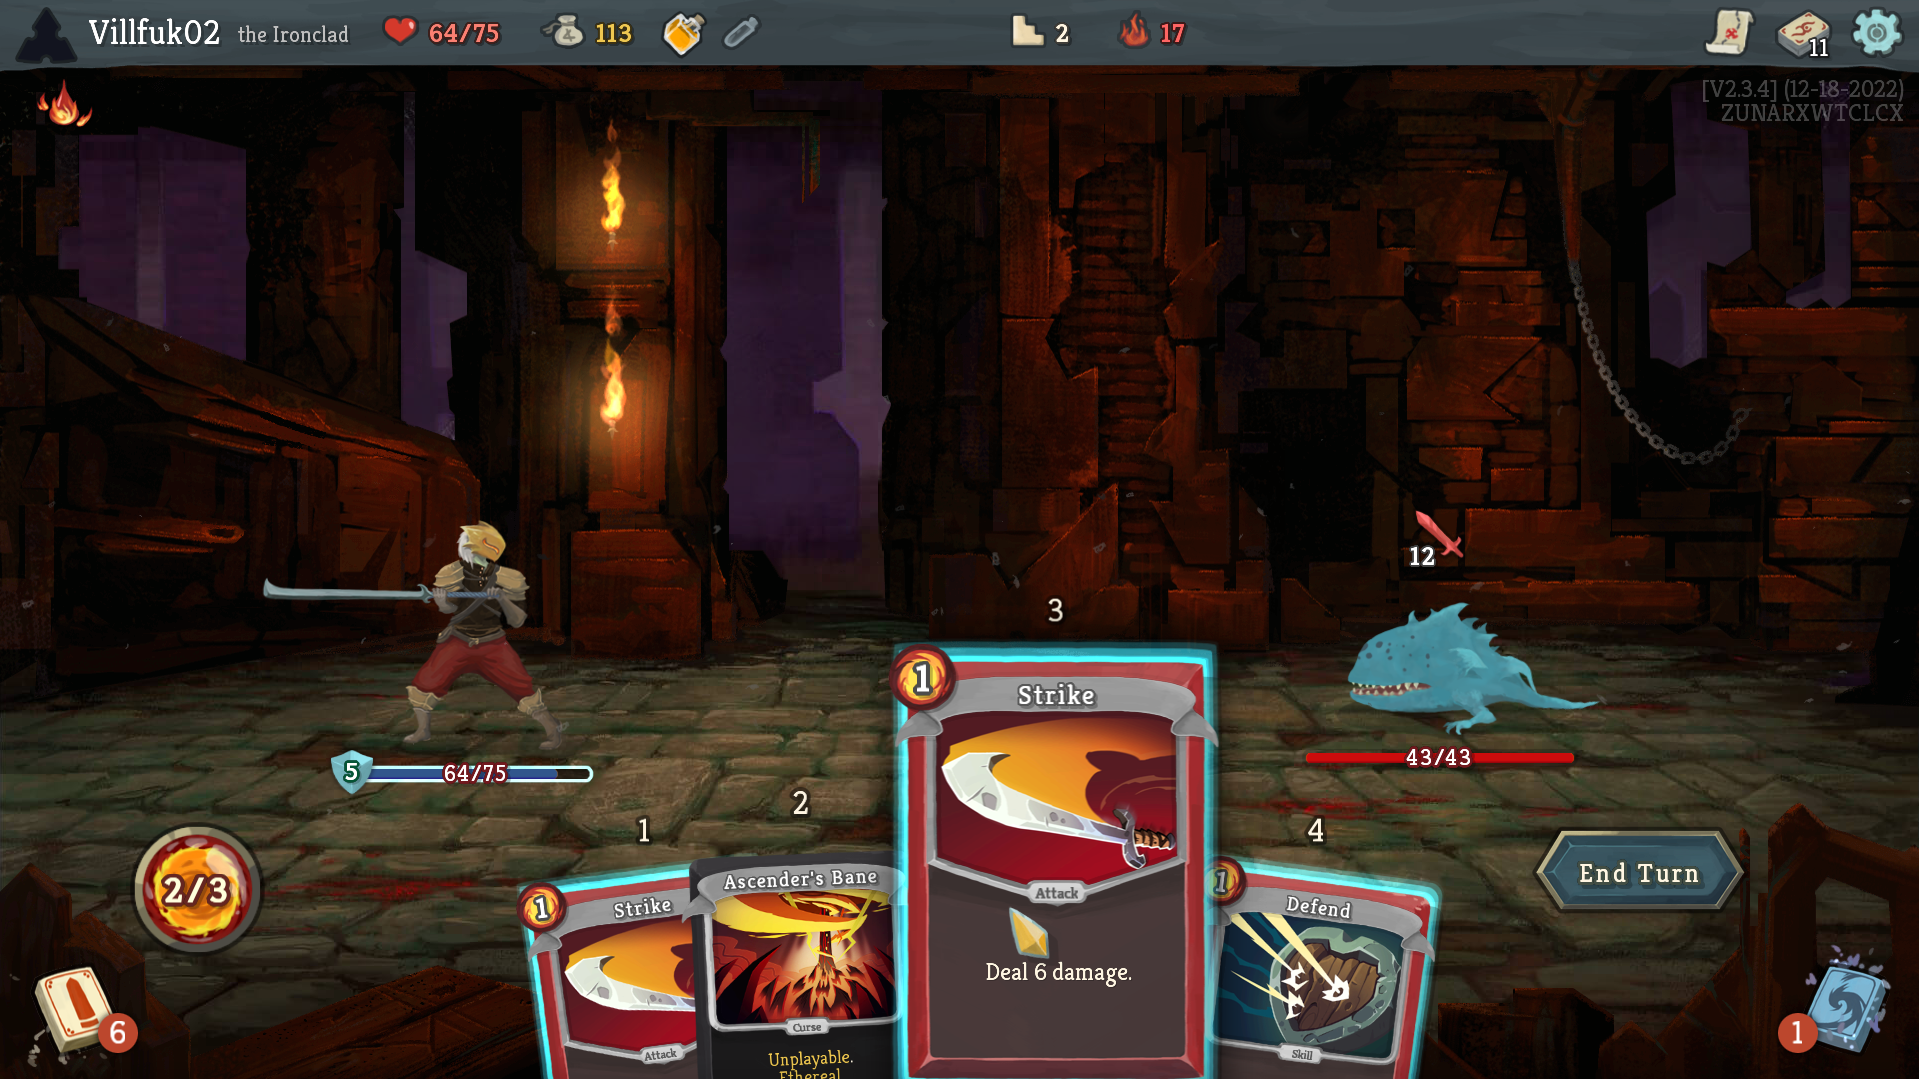
\includegraphics[width=0.8\textwidth]{img/Slay-the-Spire-Fight.png}
    \caption{A fight in Slay the Spire.}
    \label{fig:slay-the-spire-fight}
\end{figure}

\begin{figure}[htb]
    \centering
    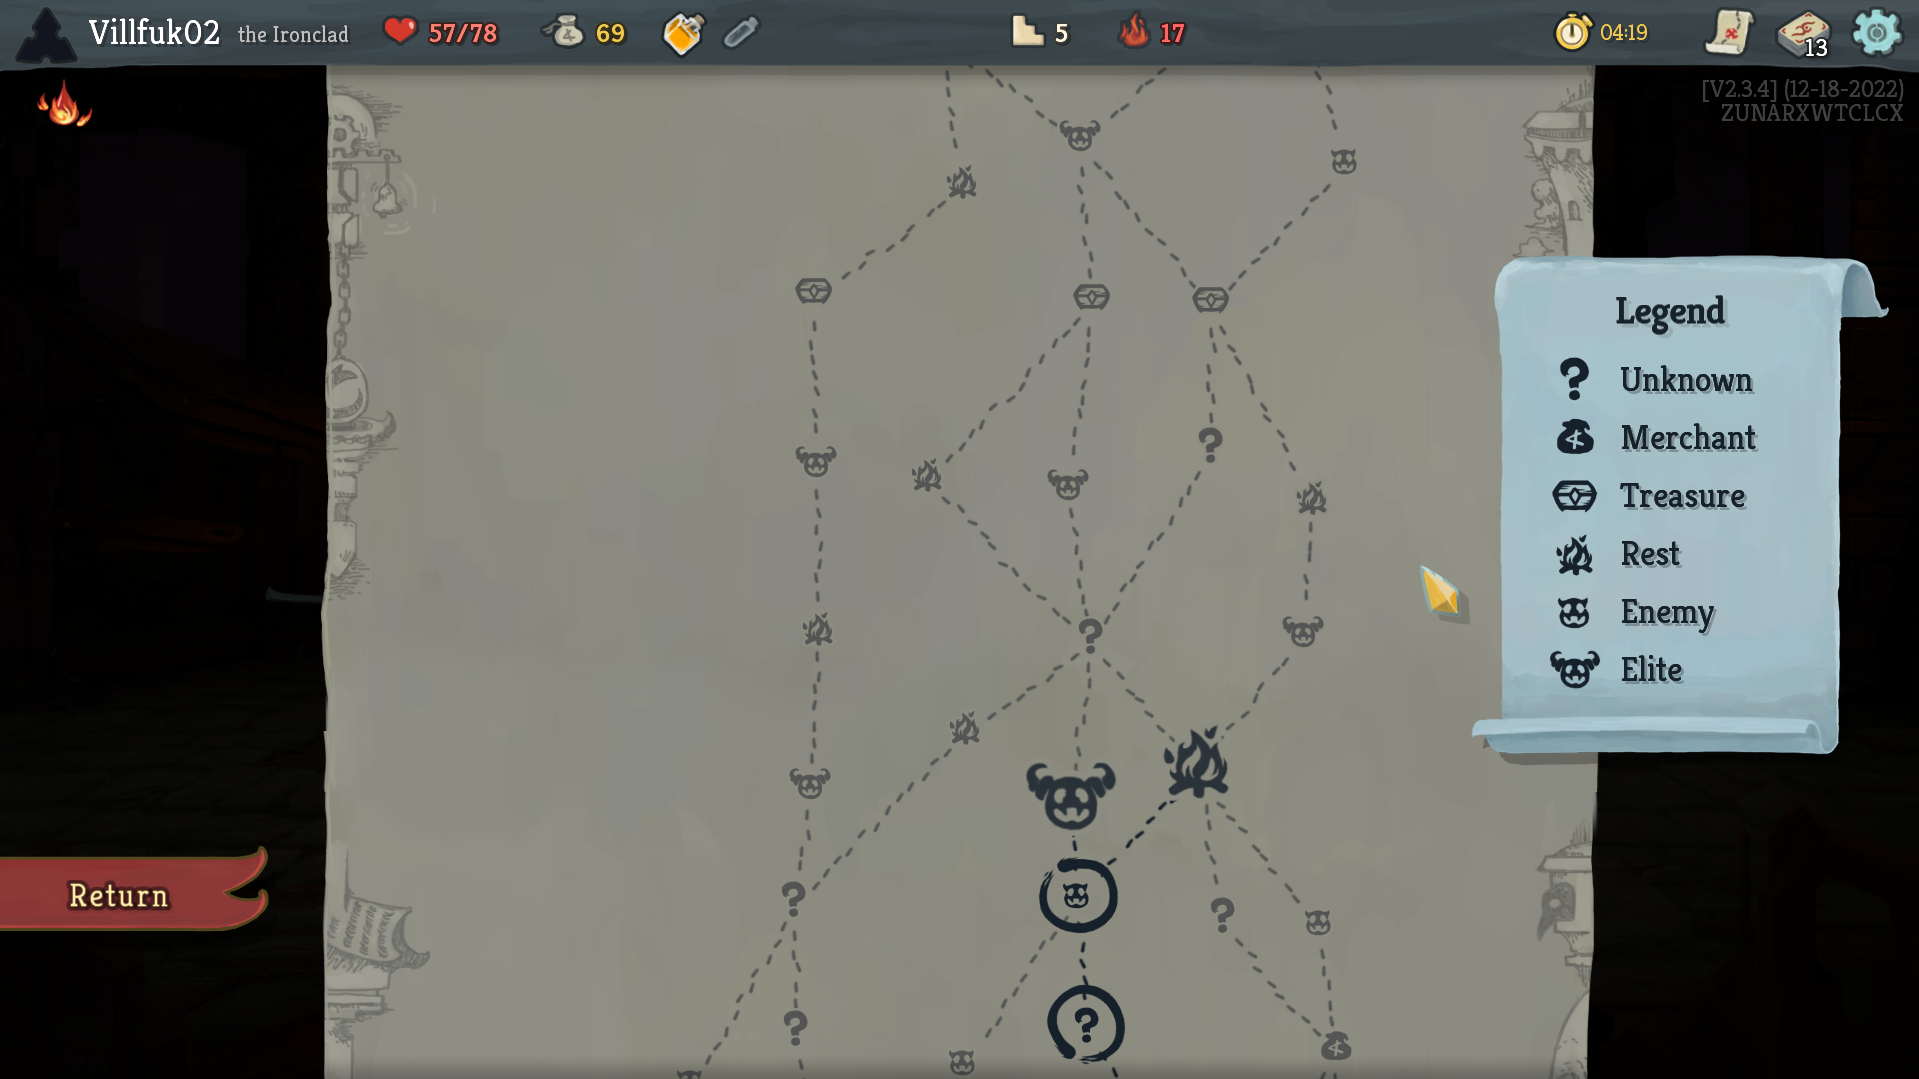
\includegraphics[width=0.8\textwidth]{img/Slay-the-Spire-Map.png}
    \caption{Slay the Spire --- map screen.}
    \label{fig:slay-the-spire-map}
\end{figure}

\subsection{Plants vs. Zombies}

- explain the game, use the following images

\begin{figure}[htb]
    \centering
    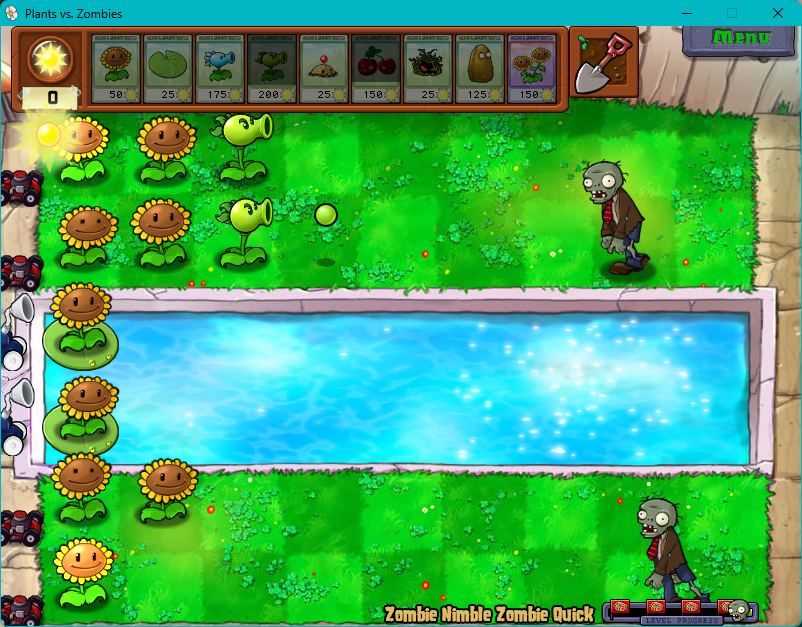
\includegraphics[width=0.8\textwidth]{img/Plants-vs-Zombies-Fight.png}
    \caption{A plants vs. Zombies level.}
    \label{fig:plants-vs-zombies-fight}
\end{figure}

\subsection{Strategic Depth in Each Battle}

- StS --- you have to balance defense and offense --- some enemies get stronger throughout the fight - refer to the fight image

- PvZ --- you have to balance defense and economy --- in each level, you want plants that help you in the short term while you build your economy and plants which are more expensive, but effective once you can afford them

\begin{figure}
    \centering
    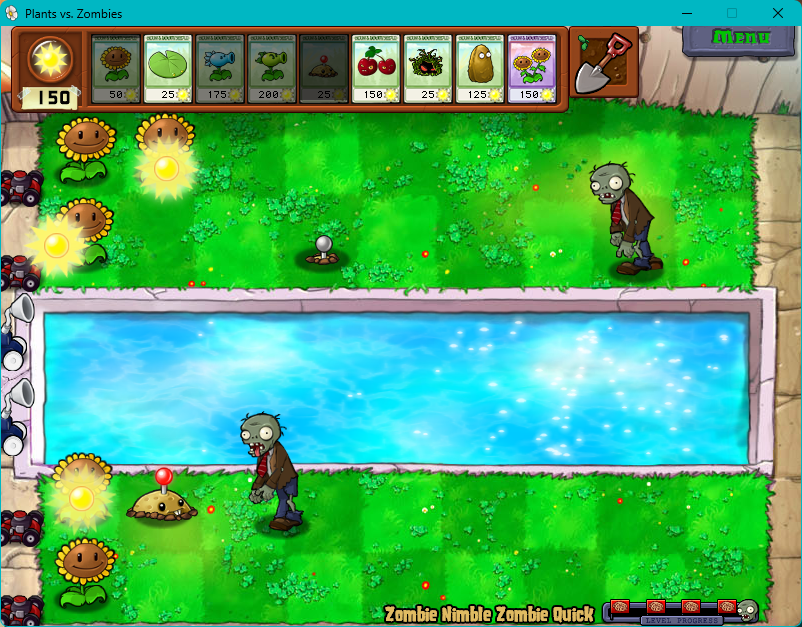
\includegraphics[width=0.8\textwidth]{img/Plants-vs-Zombies-Mines.png}
    \caption{Sunflowers and Potato Mines in Plants vs. Zombies. Sunflowers are necessary to fuel your economy, while Potato Mines are a cheap way to deal with the first few zombies.}
    \label{fig:plants-vs-zombies-mines}
\end{figure}

- in our game you have fuel mining as offense and defensive towers as defense, economic buildings and abilities, so you have to balance short-term and long-term power

\subsection{Strategic Depth in Each Run}

- StS --- As you get better, you realize there is this interesting trade-off between short-term and long-term power - you want cards to survive the next few fights, but they will be duds later; you also want cards which will have greater synergy in the future, but don't help you right now.

- examples - iron wave, entrench

\begin{figure}
    \centering
    \begin{minipage}{.5\textwidth}
        \centering
        \captionsetup{justification=centering}
        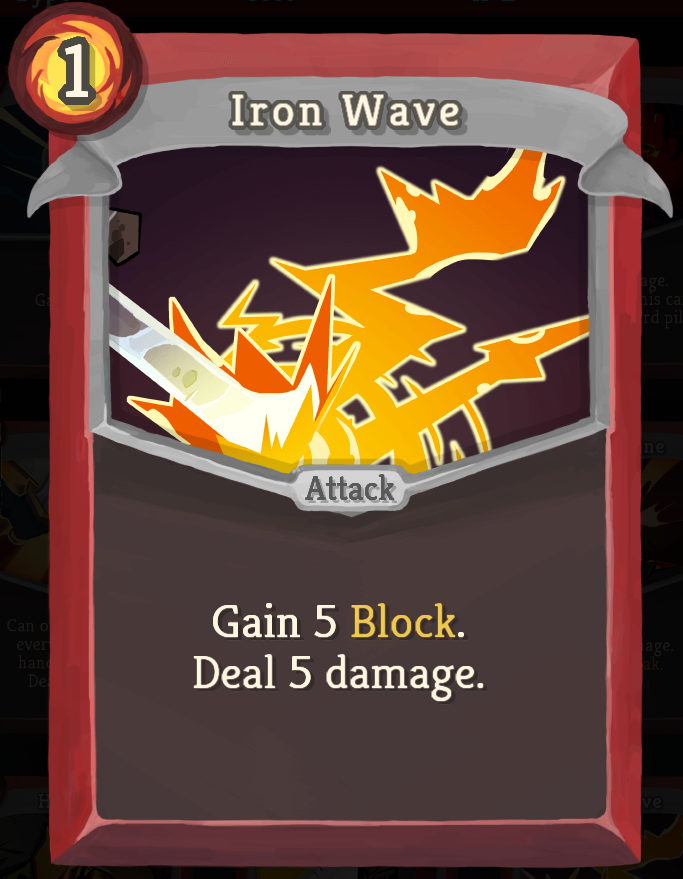
\includegraphics[width=0.5\textwidth]{img/Slay-the-Spire-Iron-Wave.png}
        \caption{Iron Wave --- a card\\in Slay the Spire.}
        \label{fig:slay-the-spire-iron-wave}
    \end{minipage}%
    \begin{minipage}{.5\textwidth}
        \centering
        \captionsetup{justification=centering}
        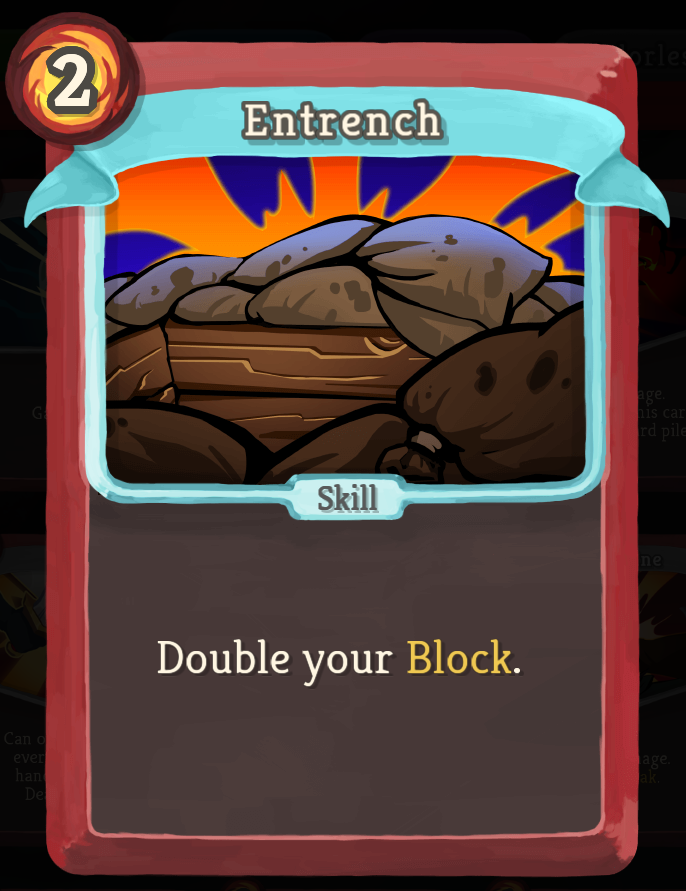
\includegraphics[width=0.5\textwidth]{img/Slay-the-Spire-Entrench.png}
        \caption{Entrench --- a card\\in Slay the Spire.}
        \label{fig:slay-the-spire-entrench}
    \end{minipage}
\end{figure}

\subsection{Make Various Strategies Viable}

- StS --- some cards interact in interesting ways that make them stronger ; there are cards and relics which fundamentally change the way your deck works (ex. barricade and entrench)

\begin{figure}[htb]
    \centering
    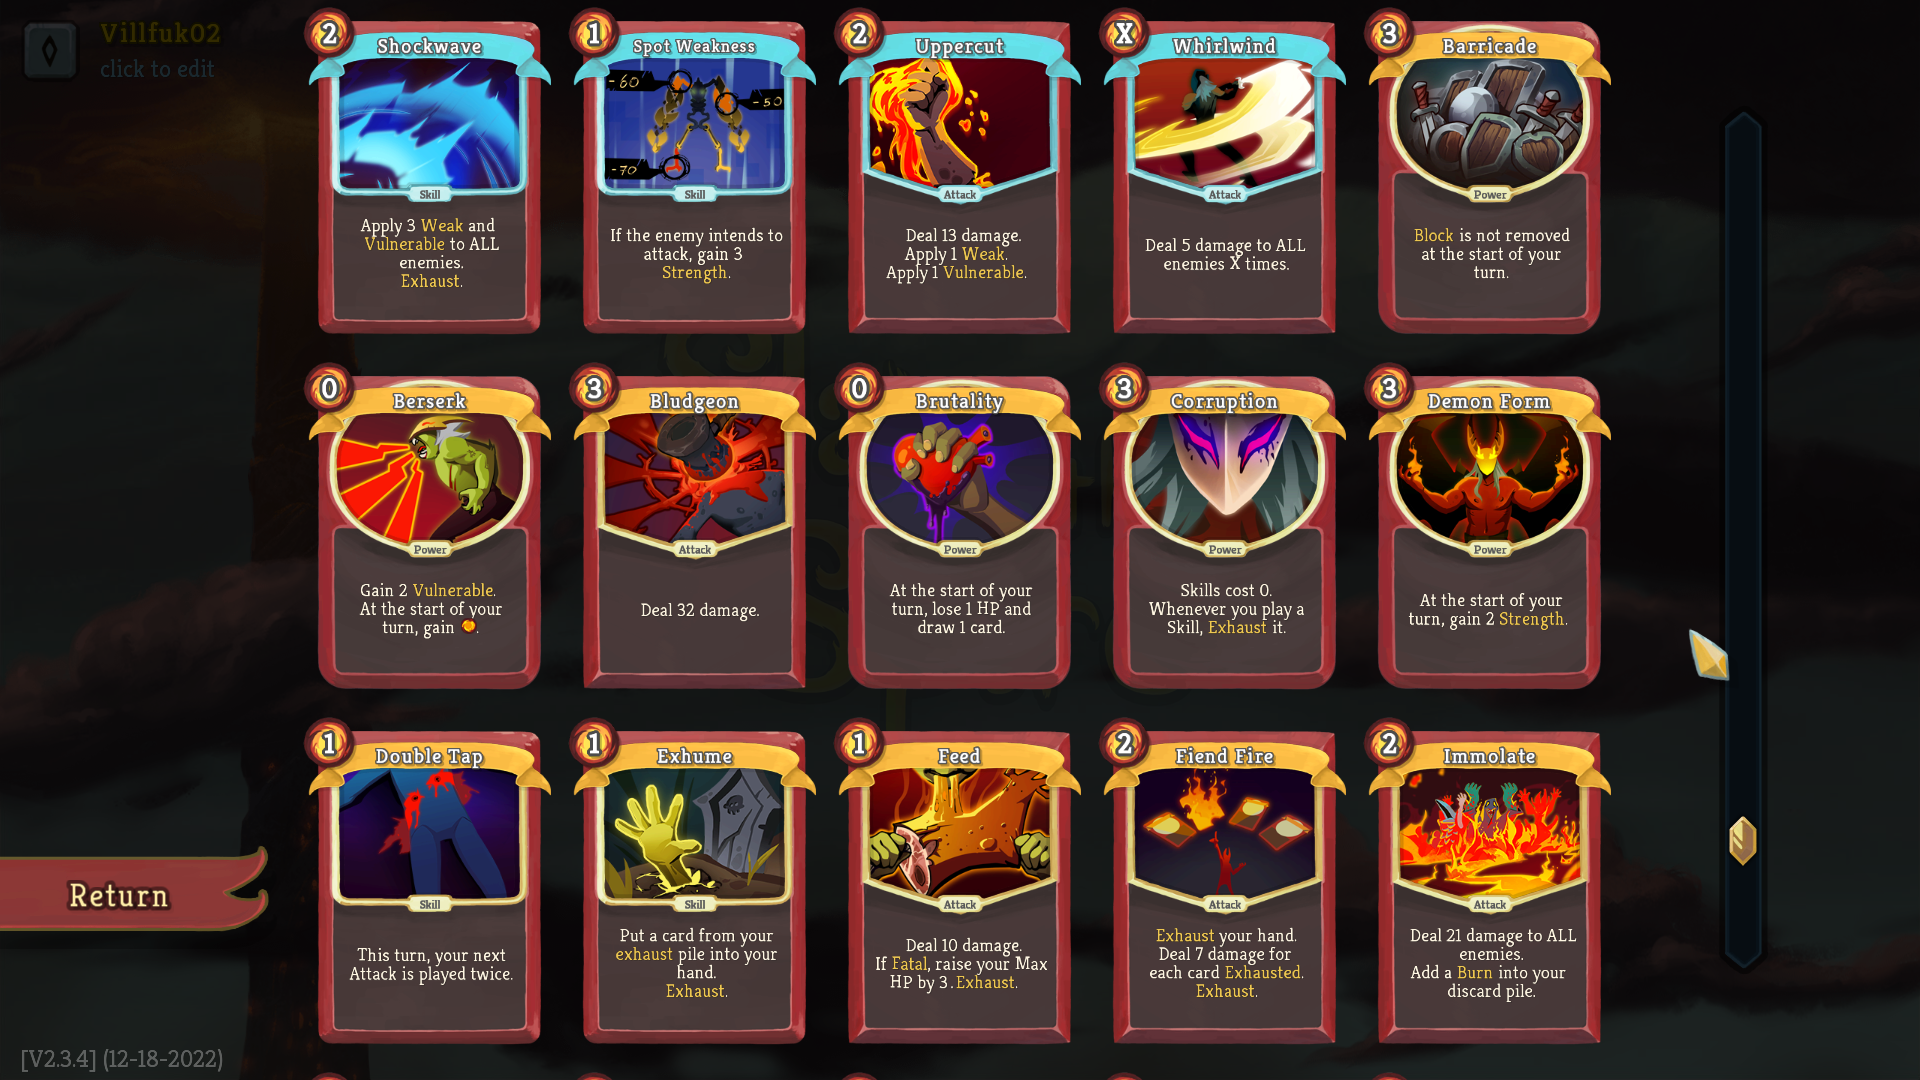
\includegraphics[width=0.8\textwidth]{img/Slay-the-Spire-Compendium.png}
    \caption{A small portion of the many interesting cards in Slay the Spire.}
    \label{fig:slay-the-spire-compendium}
\end{figure}

- PvZ --- the interactions are not so strong, but you have to combine the plants such that you have no weak spots --- cheap and expensive, for specific zombie types

\begin{figure}[htb]
    \centering
    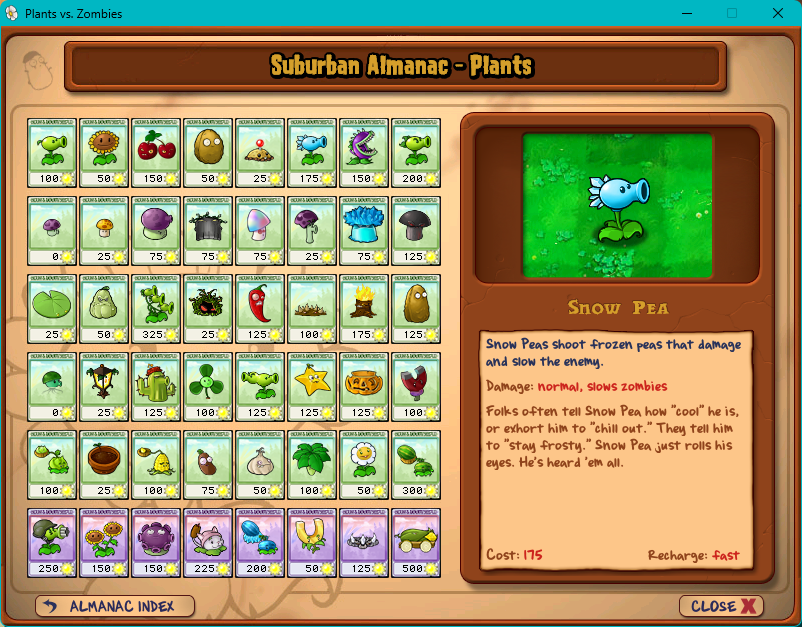
\includegraphics[width=0.8\textwidth]{img/Plants-vs-Zombies-Almanac.png}
    \caption{All the plants of Plants vs. Zombies in the in-game almanac.}
    \label{fig:plants-vs-zombies-almanac}
\end{figure}

- make blueprints that have unique effects that change the way you play

\subsection{Force Exploration}

- StS --- you have to explore different strategies because you get different cards every time, some enemies ensure you are prepared for everything and intentionally break some strategies

- characters

\begin{figure}[htb]
    \centering
    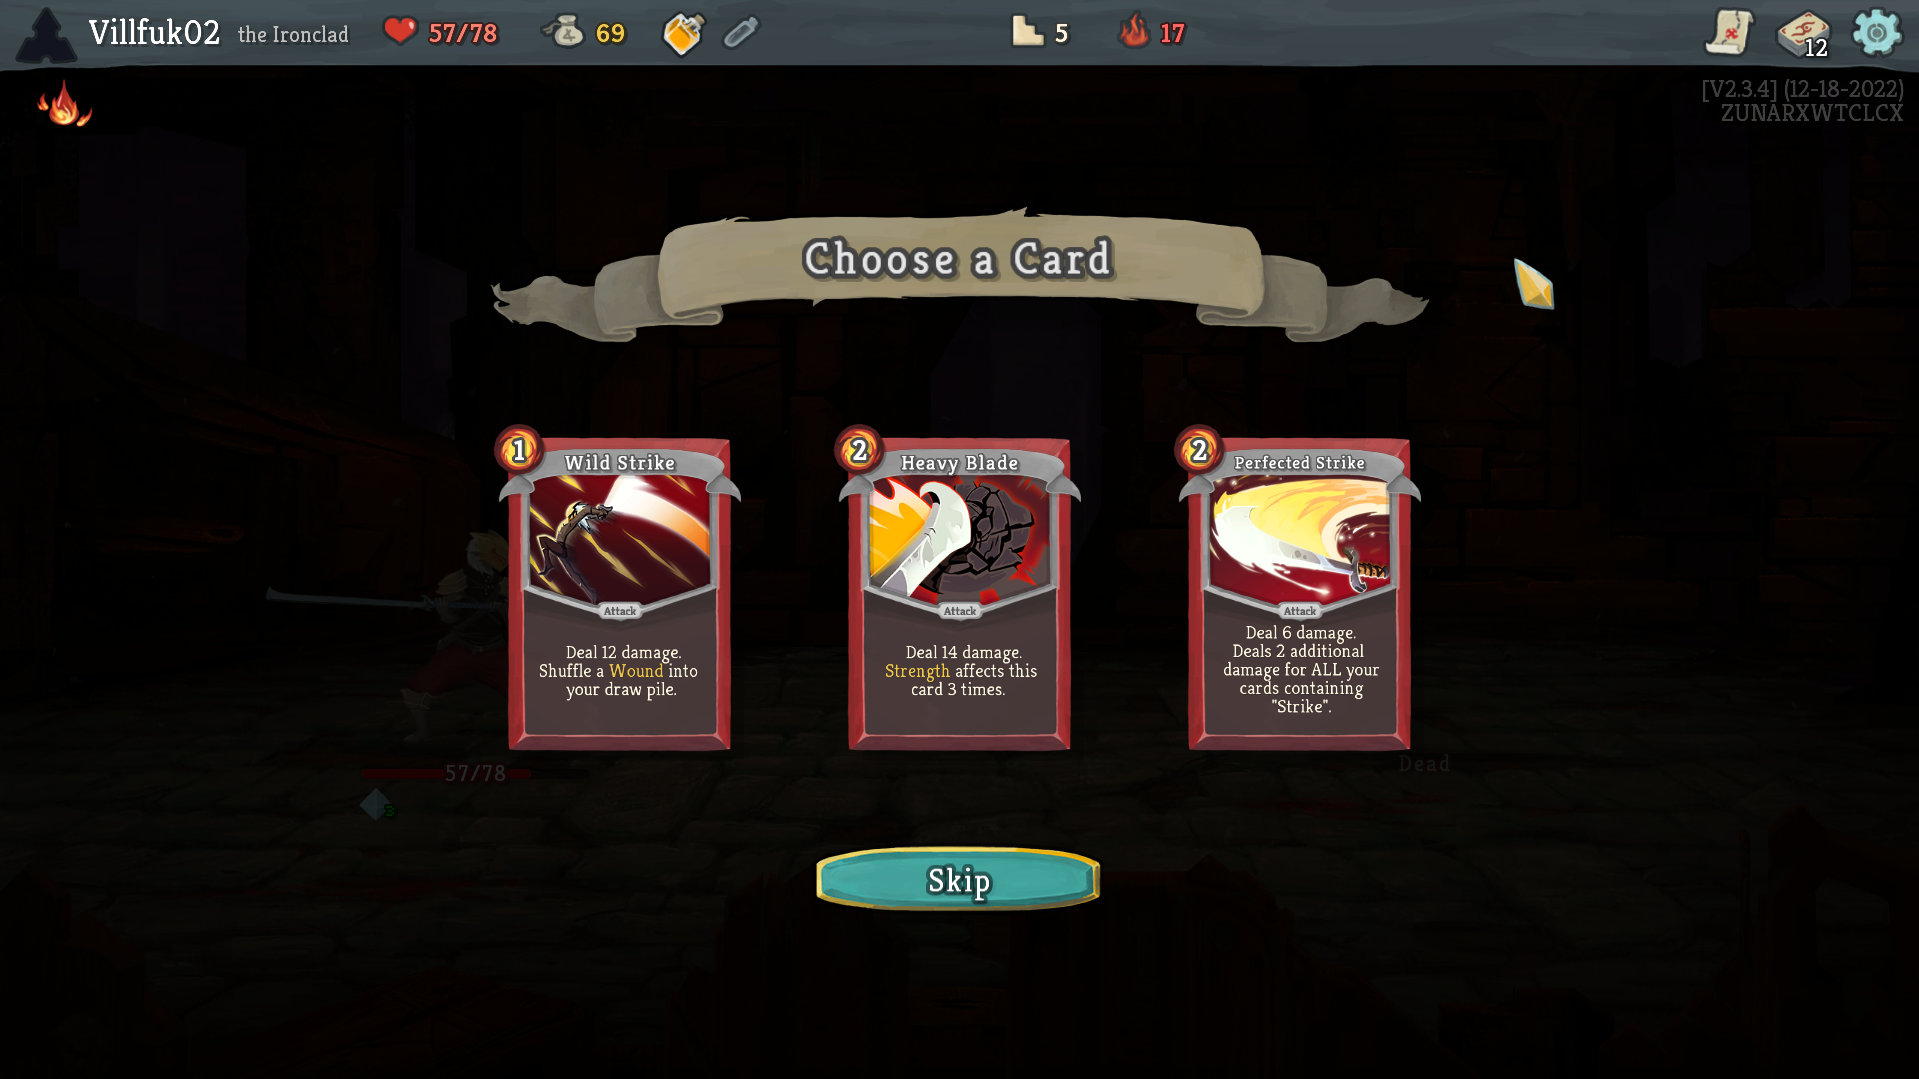
\includegraphics[width=0.8\textwidth]{img/Slay-the-Spire-Reward.png}
    \caption{Card reward screen in Slay the Spire. Here the player can choose on of three randomly selected cards to add to their deck.}
    \label{fig:slay-the-spire-reward}
\end{figure}

- PvZ --- you have to explore different strategies because you have to adapt to different zombies and level environments, not too deep; after the campaign, three seed slots are selected for you.

\begin{figure}[htb]
    \centering
    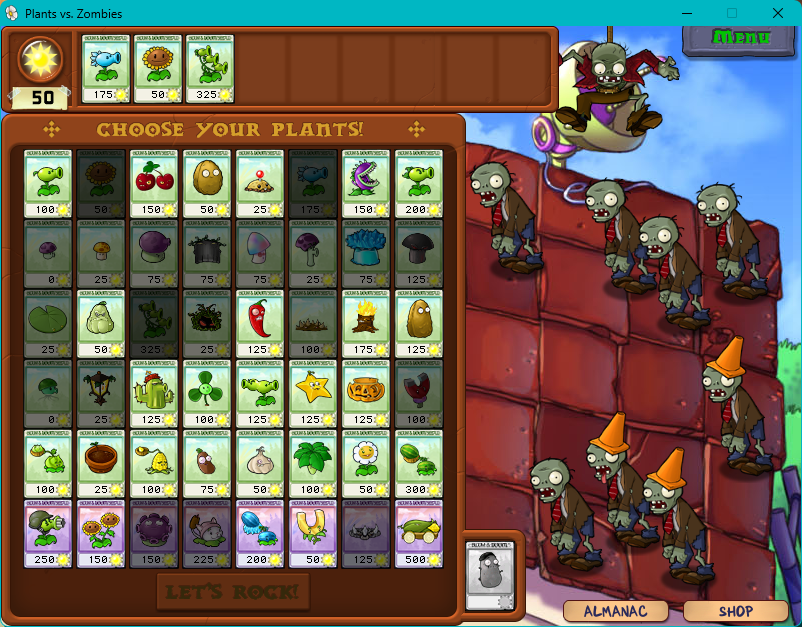
\includegraphics[width=0.8\textwidth]{img/Plants-vs-Zombies-Rooftop.png}
    \caption{Seed select screen in a rooftop level. Here, plants must be planted in flower pots, and most plants cannot shoot uphill.}
    \label{fig:plants-vs-zombies-roof}
\end{figure}

- choose from random blueprints, various attackers with abilities and terrain types

\subsection{Provide a Challenge}

- StS --- not easy to beat; after you beat the game, you can play on a higher ascension

\begin{figure}
    \centering
    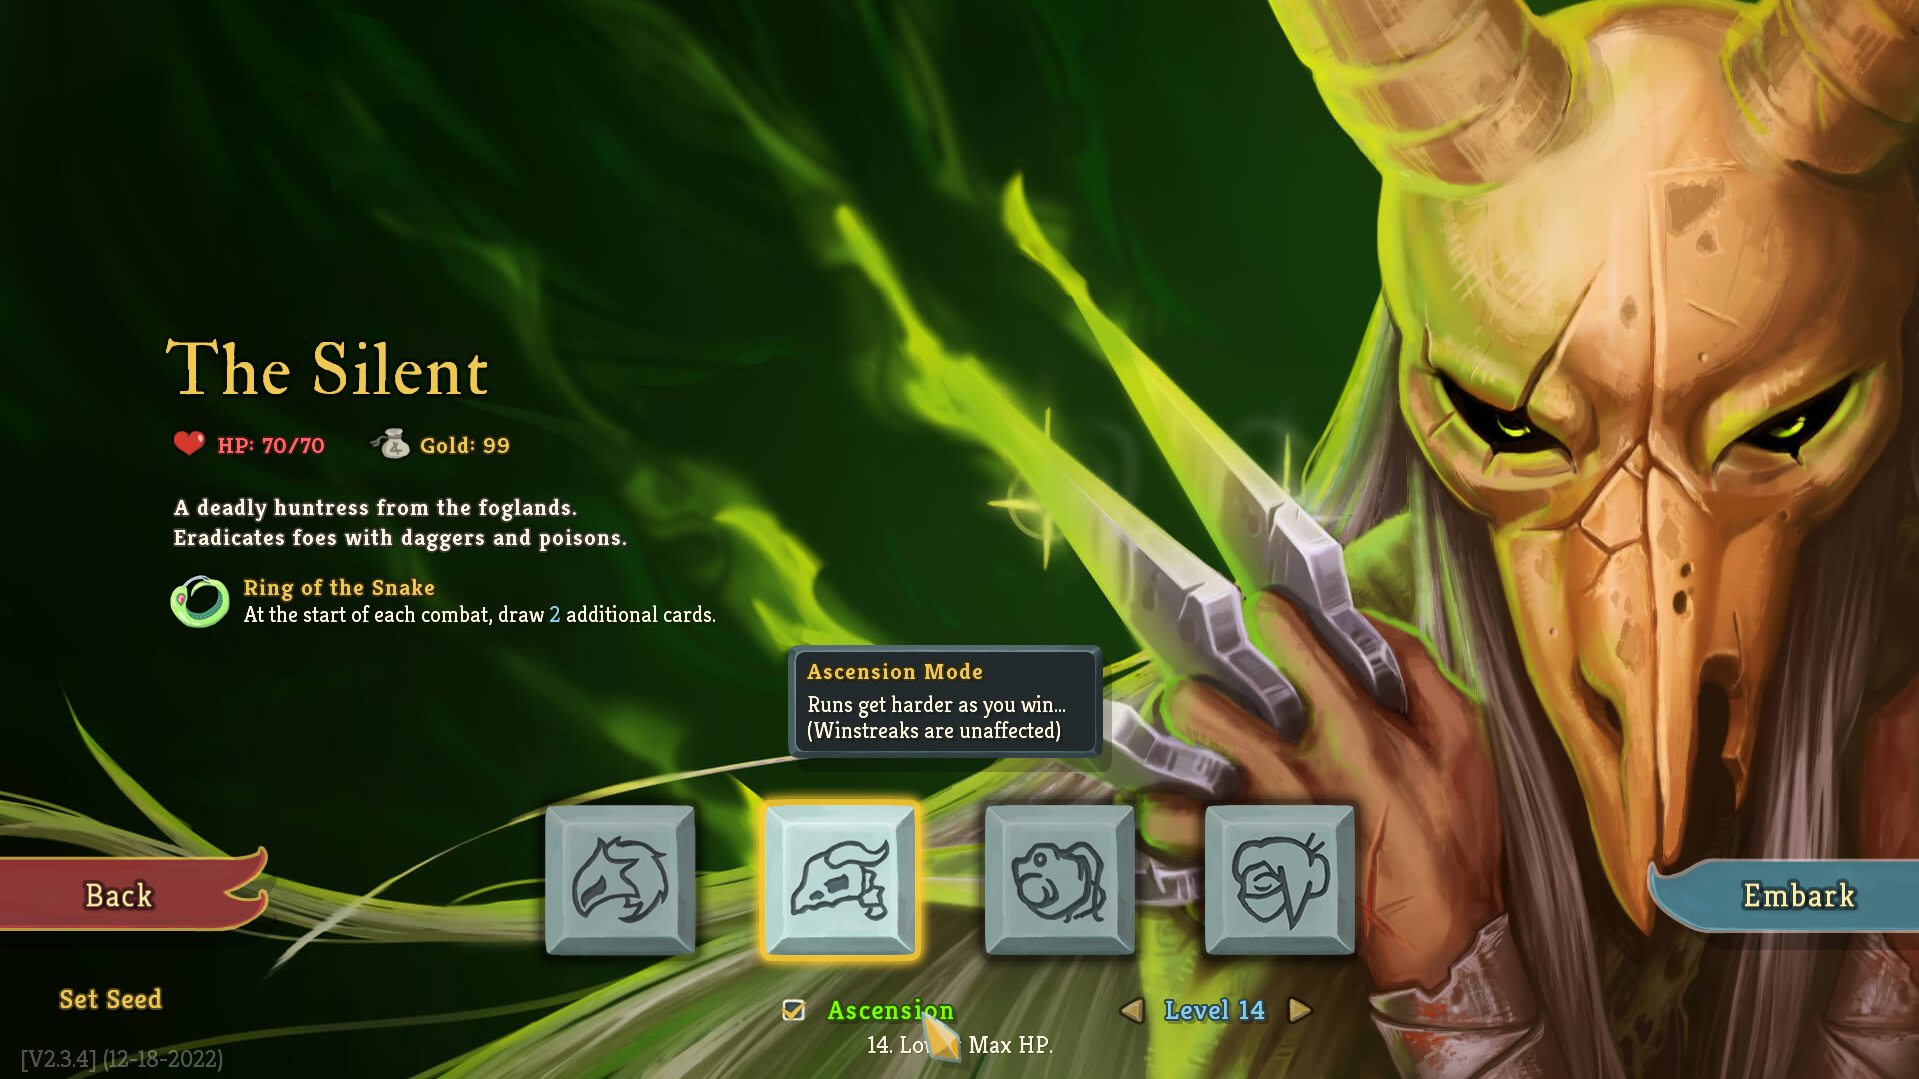
\includegraphics[width=0.8\textwidth]{img/Slay-the-Spire-Ascension.png}
    \caption{Character select screen in Slay the Spire. Here the player can also choose their ascension level, making the game harder.}
    \label{fig:slay-the-spire-ascension}
\end{figure}

- we will have something similar to StS

\section{Battle}

- overview viz \autoref{sec:original-vision}

- build stuff, send waves, use abilities

\section{Attacker Movement}

- free movement with individual pathfinding X

- too unpredictable for the player --- The player needs to plan in advance in order to maximize the possibility to take calculated risks
- solution: visualize enemy paths --- Too many different paths - too much clutter; Still planning at most one wave in advance

- linear lanes (like in Plants vs. Zombies) X
- not enough space for interesting building placement

- paths based on your buildings X
- what if they block off the path?

- predefined paths \checkmark

- branching

\section{World}

- free placement X

- grid of tiles \checkmark
- more granularity, easier to develop intuition, same for attacker paths

- hexagons X

- squares \checkmark

- 3D \checkmark
- Simple and intuitive way to make the level itself more interesting
Some towers won't be able to shoot uphill or downhill - more interesting decisions for the player

- Terrain types

- Obstacles

\section{Resources}

\subsection{Materials}

\subsection{Energy}

\subsection{Hull}

\section{Graphical User Interface}

\todo{specify controls}

\subsection{Waves Left and Fuel}

\subsection{Hull}

\subsection{Wave Preview}

\subsection{Materials and Energy}

\subsection{Blueprints}

- what they represent

- rarities

- make them unique

- lenticular design

\subsection{Info Panel and Selection}

- what it looks like and what's on it

- select blueprints

- select buildings

- select attackers

\subsection{Highlights and Range Visualization}

\section{Attackers}

- move, have health

- sizes

- special abilities - passive, repeating, reactive

\section{Buildings}

- how and when to build, one per tile

- special building have special abilities

- main types:

\subsection{Economic buildings}

-provide resources

\subsection{Towers}

- attack attackers

- range

- targeting

- projectile types

- damage types

\section{Abilities}

- used mid-wave

- usually instant effects

- free placement, global placement, tile placement, use on a building

\section{Camera controls}

- zoom to look closely, rotate so the terrain doesn't hide stuff

\section{Future Features}

- run structure

- map

- events and shops

- difficulty levels

- unlocks
